\section{Introduction}
\label{sec:introduction}
\lhead{\thesection \space Introduction}

This document is the personal development plan of the author in the context of the module \textit{Software Factory}, which is part of the Software Engineering course at Fontys Hogeschool Techniek en Logistiek Venlo. As part of this module, students taking part in the course have to define their own competences regarding activities taking place in a software development project and the level of competence they want to achieve during the course of the project that makes up the \textit{Software Factory} module. The author takes the role of \textit{Software Architect} in the project group.
\newline
To define competences, this report makes use of the model used to describe the Bachelor of ICT, which includes a competence matrix known as \textit{Body of Knowledge and Skills} (BOKS), as seen in Figure \ref{fig:boks}. This matrix includes both the activities as well as the architectural layers common in an ICT environment as its dimensions. Each combination of activity and architectural layer makes up a form of competence, which can be ranked in level of skill, on a scale of 1 to 3.

\begin{figure}[!ht]
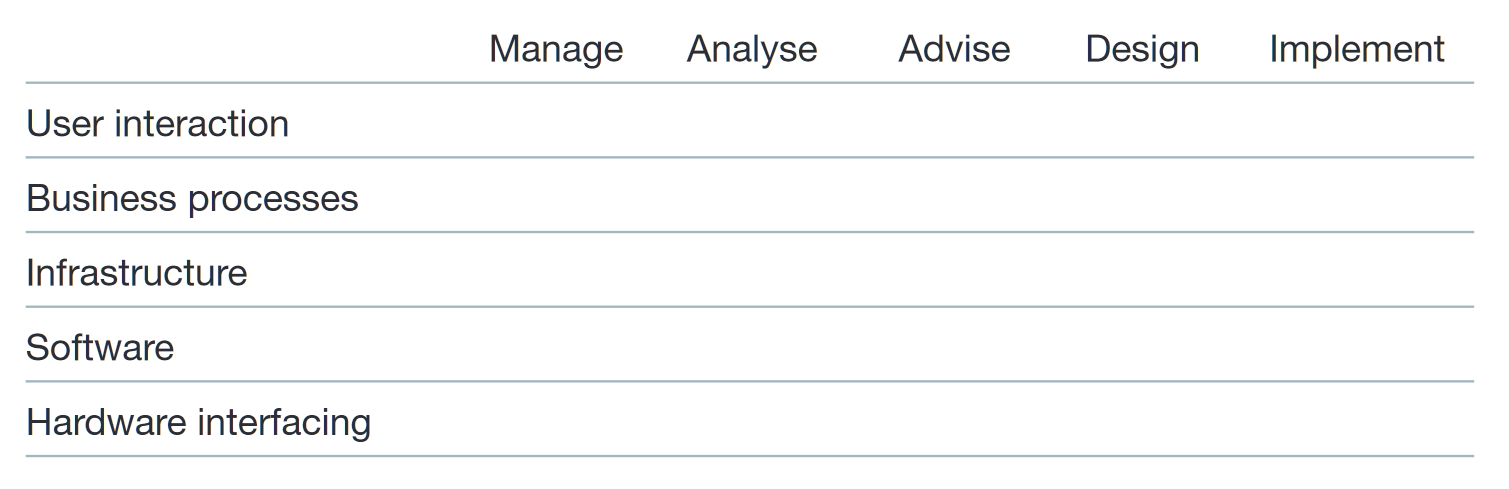
\includegraphics[width=\textwidth]{Pics/boks.png}
\caption{Body of Knowledge and Skills}
\label{fig:boks}
\end{figure}

This report will cover three activities in a certain architectural layer listed in the Figure above. To do so, it will be described what level of competence the author possesses in executing each activity in one certain architectural layer. It is described what level the competence represents and why this current level of competence is justified. Furthermore, it is detailed how the author plans to develop their skill set to increase their level of competence to 3. For each activity and architectural layer it is described what is necessary to qualify for such a level of competence and how the author wishes to learn these skills in the context of the project. Since meeting these learning goals by the end of the project is the responsibility of the author, it will also be detailed how the author would like to prove that they have advanced their skills in the mentioned context.